\documentclass[a4paper,12pt]{article}

% Module de base utf, français
\usepackage[utf8]{inputenc}
\usepackage[T1]{fontenc}
\usepackage[french]{babel}
% gestion des marges
\usepackage[top=2cm, bottom=2cm, left=2cm, right=2cm]{geometry}

% quote
% \usepackage{csquotes}

% Packages math
%\usepackage{amsmath}
%\usepackage{amssymb}
%\usepackage{mathrsfs}

% Package tableau
\usepackage{multirow}

% Package insertion d'image
\usepackage{graphicx}
\usepackage{float}
\usepackage{subcaption} %image multiple

% Package url
\usepackage{url}	

% Package de couleur
\usepackage{color}
\usepackage[colorlinks,linkcolor=black,urlcolor=blue]{hyperref}

% Package pour le code, nécessite package color
\usepackage{listings}
\usepackage{amsmath}
\lstset{ % General setup for the package
	language=Python,
	basicstyle=\small\sffamily,
	numbers=left,
 	numberstyle=\tiny,
	frame=tb,
	tabsize=4,
	columns=fixed,
	showstringspaces=false,
	showtabs=false,
	keepspaces,
	commentstyle=\color{red},
	keywordstyle=\color{blue},
	breaklines=true
}

% Packages Verbatim
\usepackage{moreverb}

% nouvelle commande pour ~
%\newcommand{\tidle}{\char`\~}

\title{Projet L3\\Fouille de données\\Ingénierie des langues}
\author{GOEHRY Martial\\16711476}

\begin{document}
	\maketitle
	\tableofcontents
	\newpage
	
	\section*{Introduction}
		\subsection*{Mise en place de l'infrastructure opérationnelle}
	
	\section{Fouille de données}
		\subsection{Récolte des données}
		\subsection{Pré-traitement}
			\subsubsection{Extraction du corps des mails}
			\subsubsection{Nettoyage}
		\subsection{Mise en base}
	
	\section{Ingénierie des langues}
		\subsection{Recherche des caractéristiques}
			\subsubsection{Analyse statistique}
		
		\subsection{Traitement du langage}
			\subsubsection{Lemmatisation}
			\subsubsection{Vectorisation}
	
	\section{Modélisation}
		\subsection{Entraînements}
		\subsection{Validation}
		
	\section{Conclusion}
	
	
	\appendix	
	\section{Développement visualisation distribution de Zipf}
	\label{sec:devZipf}
	\paragraph{Présentation}
		La loi de distribution de Zipf est une loi empirique (basée sur l'observation) qui veut que le mot le plus fréquent est, à peu de chose près, 2 fois plus fréquent que le $2^{eme}$, 3 fois plus fréquent que le $3^{eme}$ etc.\\
		
		La formulation finale de la $1^{ere}$ loi de Zipf est la suivante :
		
		\begin{align*}
				|mot| = constante \times rang(mot)^{k \approx 1}
		\end{align*}
		
		avec \emph{$|mot|$} la fréquence d'apparition d'un mot, \emph{constante} une valeur propre à chaque texte, \emph{rang(mot)} la place du mot dans le tri décroissant par fréquence d'apparition et \emph{k} un coefficient proche de 1. 
		
	\paragraph{Développement}
		Afin de pouvoir utiliser les résultats de cette distribution dans ce projet, j'ai développé un ensemble de fonctions sur un corpus "\emph{reconnu}". Mon choix s'est porté sur le corpus \emph{Brown} (voir \ref{Brown_corpus}) présent dans la librairie \emph{nltk}. Ce corpus contient environ 500 documents contenant 1 millions de mot en anglais.\\
		
		Le processus d'analyse se fait sur 2 versions de ce corpus.
		\begin{itemize}
			\item la première version contient tous les mots sans modifications
			\item le seconde version contient tous les mots sans les \emph{stopwords}
		\end{itemize}
		Les \emph{stopwords} sont des mots qui n'ont pas ou peu de signification dans un texte. Ces mots sont retirés dans la $2^e$ version pour voir l'effet d'une réduction sur la distribution de Zipf. \\
		
		Les paragraphes ci-dessous détaillent les étapes du développement :
		
		\subparagraph{Étape 1 - Ordonner les mots}
			La première étape est de compter les occurrences de tous les mots des 2 corpus et de les ranger en fonction de leur nombre d’occurrence. 
			\begin{lstlisting}[title=Triage des mots]
def frequence_mot(bag, freq=None):
    """
    Calcule la frequence de chaque mot dans un sac de mot
    :param bag: <list> - liste de tous les mots d'un texte
    :param freq: <dict> - dictionnaire avec {<str> mot: <int> frequence}
    :return: <dict> - dictionnaire avec la frequence par mot {mot: frequence}
    """
    if freq is None:
        freq = {}
    for mot in bag:
        freq[mot] = freq.get(mot, 0) + 1
    return freq
		
def classement_zipf(dico):
    """
    Trie un dictionnaire de mots : occurence et leur assigne un rang en fonction du nombre d'occurence
    :param dico: <dict> dictionnaire de mot: occurrences
    :return: <list> {"rang": <int>, "mot": <str>, "frequence": <int>}
    """
    ranked = []
    for rang, couple in enumerate(sorted(dico.items(), key=lambda item: item[1], reverse=True), start=1):
        ranked.append({"rang": rang,
                       "mot": couple[0],
                       "frequence": couple[1]})

    return ranked \end{lstlisting}
    
    		
    		On obtient les représentations suivantes: 
		\begin{figure}[H]
				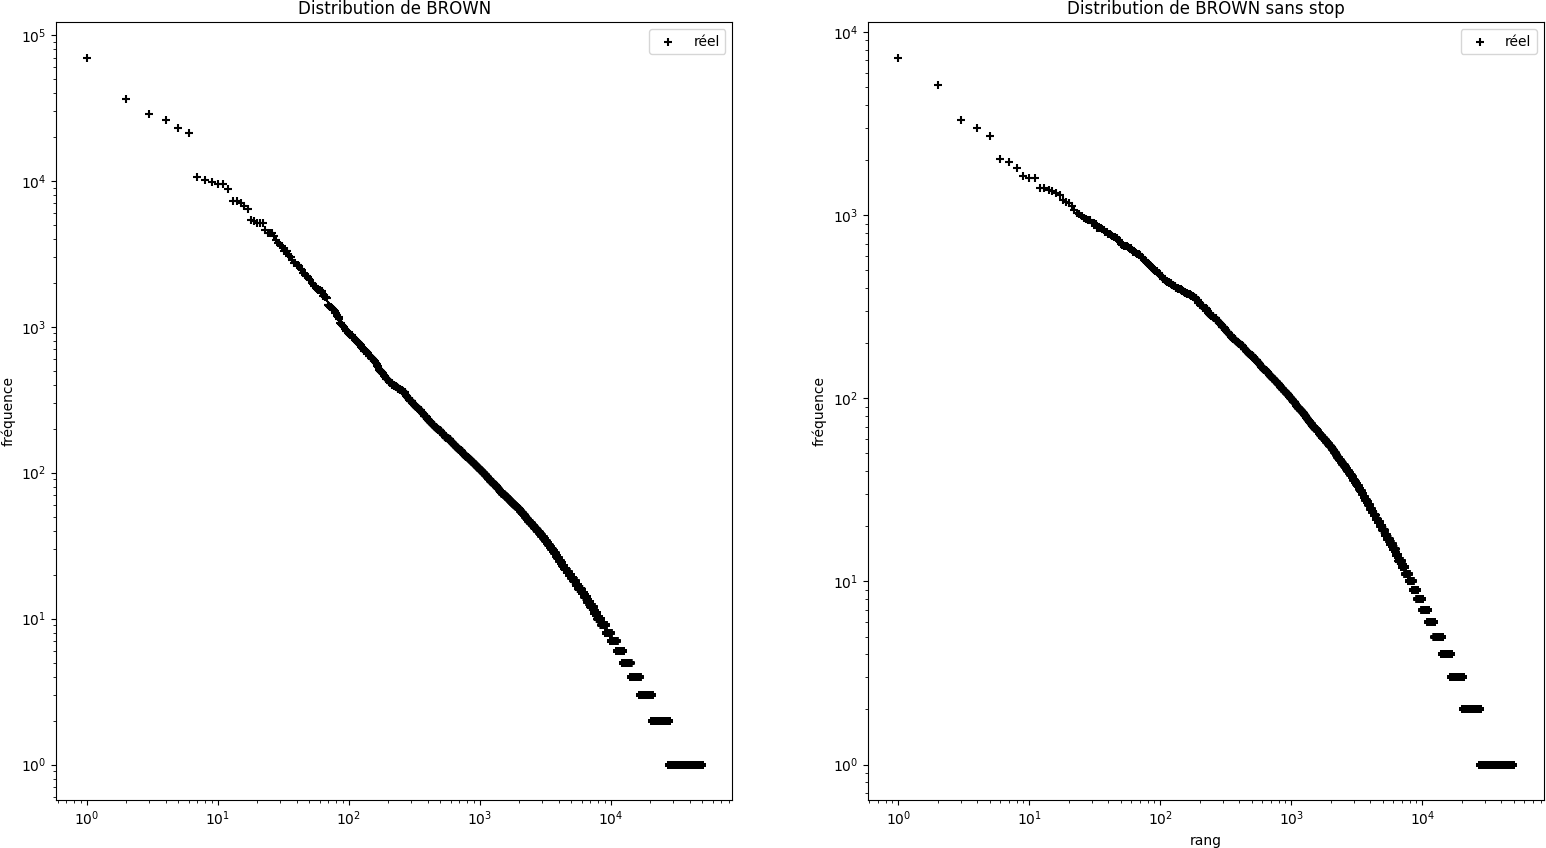
\includegraphics[width=\linewidth]{img/distribZipf.png}
				\caption{Distribution de Zipf pour les deux corpus}
		\end{figure}    		
    		
    		\begin{itemize}
    			\item Nombre de mots dans brown:	mots: 49398	occurences: 1012528
    			\item Nombre de mots dans brown stop:	mots: 49383	occurences: 578837\\
    		\end{itemize}
    		
    		La distribution de la version complète du corpus semble à première vue plus fidèle à la représentation classique de la distribution de Zipf. 
			
		\subparagraph{Etape 2 - calcul de la constante}
			Le premier paramètre qu'il faut déterminer est la \emph{constante}. Pour ce faire j'effectue le calcul suivant pour tous les mots :
			
			\begin{align*}
				constante = |mot| \times rang(mot)
			\end{align*}
			
			On obtient une liste de toutes les constantes théoriques pour chaque mot selon son rang.
			De cette liste, nous allons extraire la moyenne et la médiane.
			
			\begin{figure}[H]
				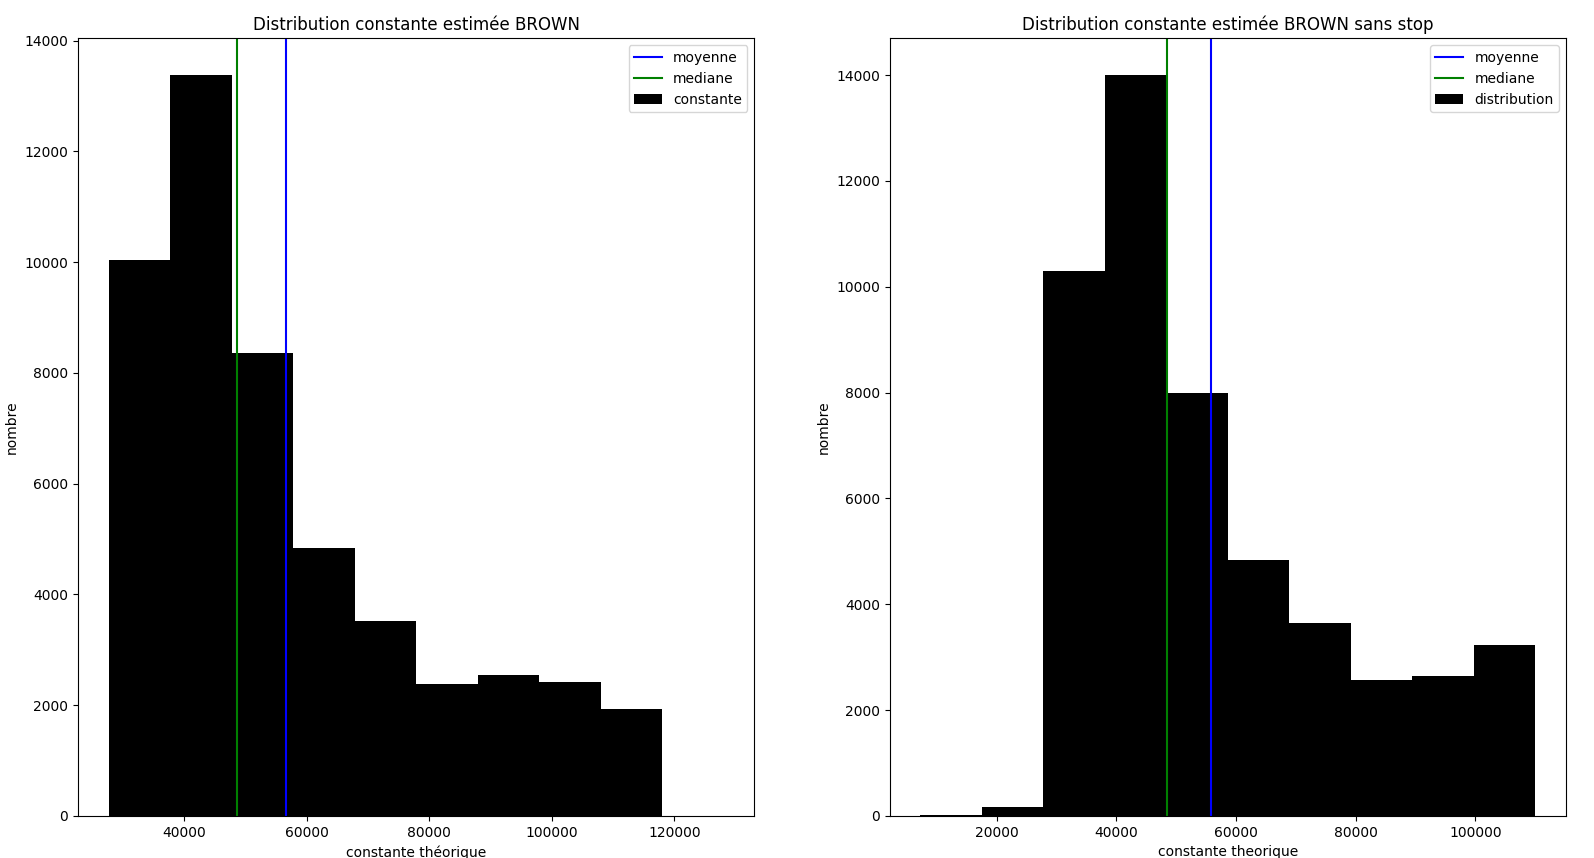
\includegraphics[width=\linewidth]{img/distribContTh.png}
				\caption{Distribution des constantes théoriques pour les deux corpus}
			\end{figure}
			
			On voit qu'il y a une majorité de mots donnant une constante brute comprise entre $20.000$ et $60.000$. Dans les deux corpus
			La différence entre les moyennes et médianes des deux corpus n'est pas flagrante :
			\begin{itemize}
				\item Brown moyenne: 56525.81, médiane: 48601.50
				\item Brown (- stopwords) moyenne: 55809.97, médiane: 48494.00
			\end{itemize}


		\subparagraph{Etape 3 - recherche du coefficient}
			Le coefficient $k$ permet d'ajuster le résultat, et pourra éventuellement donner une indication de complexité. La recherche de $k$ se fera sur les deux corpus avec utilisant les moyennes et médianes.\\
			
			Pour ce faire nous allons:

			\begin{enumerate}
				\item Faire la liste de tous les coefficients possibles dans l'intervalle $[0.86, 1.3]$ avec un pas de $0.01$\footnote{les bornes et le pas sont totalement arbitraire afin d'obtenir un graphique présentable}.
				\item Calculer toutes la fréquences théoriques de tous les rangs avec tous les coefficients possibles en utilisant les constantes moyenne et médiane de chaque corpus.
				\item Calculer la moyenne des coûts absolus entre les fréquences théoriques par coefficient avec la fréquence réelle observée pour chaque corpus.\\
			\end{enumerate}
			
			Le couple coefficient/constante avec le coup minimal sera retenu pour l'utilisation dans la phase de \emph{feature engineering}. \\	
			
			\begin{lstlisting}[title=Fonctions utilisées dans la recherche du coefficient]
def zipf_freq_theorique(constante, rang, coef):
    """
    Calcul la frequence theorique d'un mot selon son rang, la constante du texte et un coeficiant d'ajustement
    :param constante: <int> constante determinee par la distribution de Zipf
    :param rang: <int> rang du mot selon sa frequence
    :param coef: <float> variable d'ajustement
    :return: <float> frequence theorique zipfienne
    """
    return constante / (rang ** coef)
    
def cout(l1, l2, methode):
    """
    Calcul le cout de l'ecart entre les elements de l1 et le l2, place par place
    :param l1: <list> liste d'entier
    :param l2: <liste> liste d'entier
    :param methode: <str> methode de calcul du cout
    :return: <float> cout selon methode
    """
    if len(l1) != len(l2):
        print("Erreur, fonction cout: l1 & l2 de taille differente", file=sys.stderr)
        return None

    if len(l1) == 0:
        print("Erreur, fonction cout: liste vide", file=sys.stderr)

    if methode.lower() not in ['absolue', 'carre', 'racine']:
        print("Erreur, fonction cout - methode '{}' inconnue".format(methode), file=sys.stderr)
        return None

    if methode.lower() == 'absolue':
        return np.mean([abs(x-y) for x, y in zip(l1, l2)])

    if methode.lower() == 'carre':
        return np.mean([(x-y)**2 for x, y in zip(l1, l2)])

    if methode.lower() == 'racine':
        return np.sqrt(np.mean([(x-y)**2 for x, y in zip(l1, l2)]))

    return None\end{lstlisting}

			\begin{lstlisting}[title=Calcul des fréquences par coefficient]
    ls_coef = list(np.arange(0.86, 1.3, 0.01))
    zbmo_th = {coef: [stats.zipf_freq_theorique(zb_const_moyen, r, coef) for r in zb_rang] for coef in ls_coef}
    zbme_th = {coef: [stats.zipf_freq_theorique(zb_const_median, r, coef) for r in zb_rang] for coef in ls_coef}
    zbmoth_cmoy = [stats.cout(zb_freq, zbmo_th[coef], 'absolue') for coef in ls_coef]
    zbmeth_cmoy = [stats.cout(zb_freq, zbme_th[coef], 'absolue') for coef in ls_coef]

    zbsmo_th = {coef: [stats.zipf_freq_theorique(zbs_const_moyen, r, coef) for r in zbs_rang] for coef in ls_coef}
    zbsme_th = {coef: [stats.zipf_freq_theorique(zbs_const_median, r, coef) for r in zbs_rang] for coef in ls_coef}
    zbsmoth_cmoy = [stats.cout(zbs_freq, zbsmo_th[coef], 'absolue') for coef in ls_coef]
    zbsmeth_cmoy = [stats.cout(zbs_freq, zbsme_th[coef], 'absolue') for coef in ls_coef] \end{lstlisting}
		
		La recherche du coefficient nous retourne les éléments suivants:
			\begin{figure}[H]
				\includegraphics[width=\linewidth]{img/coutZipf.png}
				\caption{Coût absolu moyen par coefficient}
			\end{figure}
		
			\begin{itemize}
				\item Coût min brown moyenne: 5.93, median: 7.01
				\item Coût min brown (- stopwords) moyenne: 6.95, median: 6.46
				\item Coefficient min brown moyenne: 0.92, median: 0.91
				\item Coefficient min brown (- stopwords) moyenne: 0.97, median: 0.95
			\end{itemize}
				
	\paragraph{Résultats}
		
		Le tableaux ci dessous rappelle les données récupérées au long de la recherche:
		\begin{center}
			\begin{tabular}{|l|c|c|}
				\hline
				& BROWN avec stopwords & BROWN sans stopwords \\
				\hline
				nombre de mots uniques & 49398 & 49383 \\
				\hline
				nombre de mots total & 1012528 & 578837 \\
				\hline
				Constante moyenne & 56525.81 & 55809.97 \\
				\hline
				Constante médiane & 48601.50 & 48494.00 \\
				\hline
				Coefficient avec moyenne & 0.92 & 0.97 \\
				\hline
				Cout du coefficient moyenne & 5.93 & 6.95 \\
				\hline
				Coefficient avec médiane & 0.91 & 0.95 \\
				\hline
				Cout du coefficient médiane & 7.01  & 6.46 \\
				\hline
			\end{tabular}		
		\end{center}
		
		D'après les données il est possible de dire que l'on obtient de meilleurs résultats si on conserve tous les mots du corpus. Dans ce cas l'utilisation de la moyenne des constantes génère un taux d'erreur plus faible que la médiane.\\
		
		Ci-dessous la représentation des fréquences théoriques avec le coefficient optimal pour chaque corpus et chaque méthode. On voit que la courbe de la constante moyenne sur le corpus brute est celle qui suit le mieux les données réelles.
		\begin{figure}[H]
			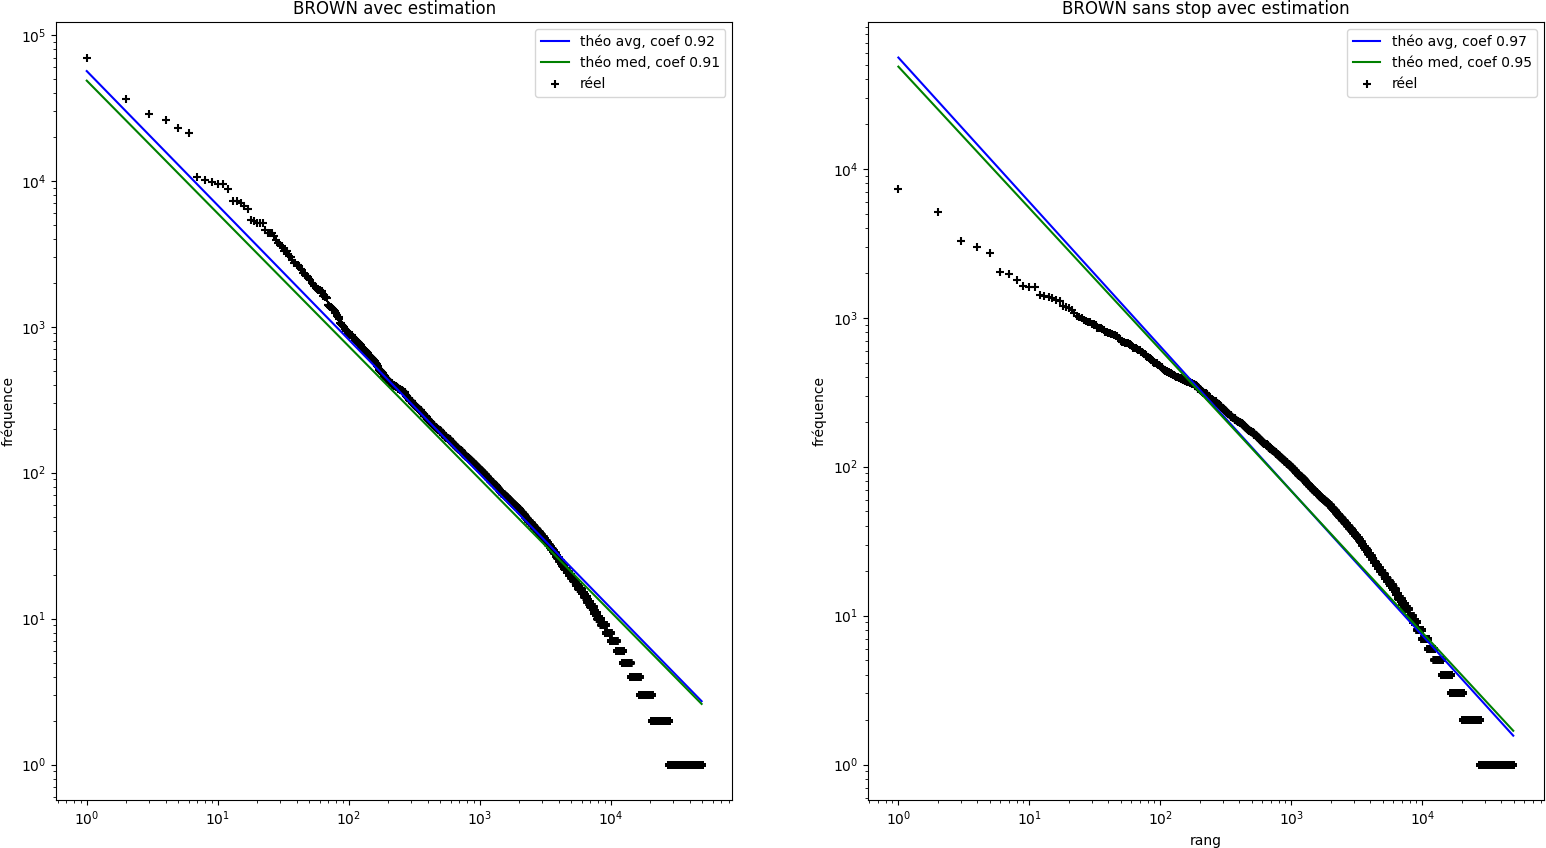
\includegraphics[width=\linewidth]{img/zipfFin.png}
			\caption{Distribution de Zipf avec les estimations}
		\end{figure}
		
		En conclusion, j'utiliserais la moyenne des constantes sur un document complet afin de déterminer le coefficient dans ma recherche de spam. 
		
		\section{Modèles}	
		\subsection{Naïves Bayes}
			Ce type de modèle est utilisé par le module \emph{langdetect} qui me sert pour la détection des langues.
			
			\paragraph{Introduction}
				Les modèles Naïves Bayes se basent sur le théorème de probabilité de Bayes. Il permet de déterminer la probabilité conditionnelle d'apparition d'un évènement A sachant qu'un évènement B s'est produit. Le terme naïf fait référence au fait que l'on présuppose que les évènements A et B ne sont pas corrélés.\\
				Ces techniques sont utilisées pour des modèles de classification en apprentissage supervisé.\\
				
				La formule mathématique de ce théorème est la suivante :
				\begin{eqnarray}\label{NBeq}
					P(A|B) &=& \frac{P(B|A)P(A)}{P(B)}
				\end{eqnarray}
				
			On recherche ici $P(A|B)$, c'est a dire la probabilité d'apparition d'un évènement A sachant que l'évènement B s'est produit. \\ 
			
			Pour ce faire nous avons besoin des données suivantes :
			\begin{itemize}
				\item $P(B|A)$ est la probabilité que l'évènement B s'est produit sachant que l'évènement A s'est produit
				\item $P(A)$ est la probabilité d'apparition de l'évènement A
				\item $P(B)$ est la probabilité d'apparition de l'évènement B
			\end{itemize}
			
			\paragraph{Exemples d'utilisation}
				Les exemples ci dessous vont permettre d'illustrer l'utilisation de cette technique. D'abord manuellement sur un petit jeu de données puis à l'aide d'un code pré-existant sur un autre jeu de données plus important.
				
				\subparagraph{Manuel}
					Dans cet exemple nous allons déterminer la probabilité qu'a un joueur d'aller sur le terrain selon les conditions météorologiques. Cette probabilité sera calculée en fonction des données récupérées lors des matchs précédents.\footnote{Les données présentées sont inventées} \\
					
					On recherchera ainsi la probabilité de présence sur le terrain d'un joueur selon la météo $P(A|B)$. Pour ce faire nous auront besoin de: 
					\begin{itemize}
						\item $P(A)$ Probabilité de jouer quelque soit le temps
						\item $P(B)$ Probabilité de l'évènement météorologique
						\item $P(B|A)$ Probabilité de l'évènement sachant que le joueur a été sur le terrain					
					\end{itemize}
				
				\begin{table}[H]
					\centering
					\captionof{table}{Données de présence sur le terrain} \label{tab:data}
					\begin{tabular}{|l|c|c|c|c|c|c|c|}
						\hline
						météo & soleil & soleil & couvert & pluie & pluie & pluie & couvert \\
						\hline
						présent & non & non & oui & oui & oui & non & oui \\
						\hline
						\hline
						météo & soleil & soleil & pluie & soleil & couvert & couvert & pluie \\
						\hline
						présent & non & oui & oui & oui & oui & oui & non \\
						\hline
					\end{tabular}
				\end{table}
				
				\begin{table}[H]
					\centering
					\captionof{table}{Synthèse et probabilité simple P(A) et P(B)} \label{tab:pab}
					\begin{tabular}{|l|c|c|r|}
						\hline
						météo & oui & non & $P(B)$\\
						\hline
						couvert & 4 & 0 & $4/14$\\
						\hline
						soleil & 2 & 3 & $5/14$\\
						\hline
						pluie & 3 & 2 & $5/14$\\
						\hline
						$P(A)$ & $9/14$ & $5/14$ & \\
						\hline
					\end{tabular}
				\end{table}
						
				On peut déterminer les probabilités de chaque météo en fonction de la présence du joueur sur le terrain P(B|A). Pour ce faire on divise le nombre d'évènements de présence du joueur lors d'un évènement météo par le nombre total d'évènements de présence du joueur
				
				\begin{table}[H]
					\centering
					\captionof{table}{Probabilité météo selon présence du joueur} \label{tab:pba}
					\begin{tabular}{|l|c|c|}
						\hline
						météo & P(B|oui) & P(B|non) \\
						\hline
						couvert & $4/9$ & $0/5$ \\
						\hline
						soleil & $2/9$ & $3/5$ \\
						\hline
						pluie & $3/9$ & $2/5$ \\
						\hline	
					\end{tabular}
				\end{table}
				
				On va maintenant calculer la probabilité qu'à un joueur d'être sur le terrain si le temps est couvert.\\
				On commence par la probabilité du oui:
				\begin{eqnarray*}
					P(A|B) &=& \frac{P(B|A)P(A)}{P(B)}\\
					P(A|B) &=& \frac{\frac{4}{9}\cdot\frac{9}{14}}{\frac{4}{14}}\\
					P(A|B) &=& \frac{\frac{4}{14}}{\frac{4}{14}}\\
					P(A|B) &=& \frac{4}{14}\cdot\frac{14}{4}\\
					P(A|B) &=& 1
				\end{eqnarray*}
				
				On enchaîne sur la probabilité de ne pas jouer si le temps est couvert
				\begin{eqnarray*}
					P(A|B) &=& \frac{P(B|A)P(A)}{P(B)}\\
					P(A|B) &=& \frac{\frac{0}{5}\cdot\frac{5}{14}}{\frac{4}{14}}\\
					P(A|B) &=& 0\cdot\frac{14}{4}\\
					P(A|B) &=& 0
				\end{eqnarray*}	
				
				On peut dire que si le temps est couvert le joueur très probablement sur le terrain			 
				On peut également déterminer la probabilité de jouer pour chaque évènement météo
				\begin{table}[H]
					\centering
					\captionof{table}{Probabilité présence du joueur selon la météo} \label{tab:pab2}
					\begin{tabular}{|l|c|c|c|}
						\hline
						météo & oui & non & plus probable\\
						\hline
						couvert & 1 & 0 & oui\\
						\hline
						soleil & 2/5 & 3/5 & non \\
						\hline
						pluie & 3/5 & 2/5 & oui \\
						\hline
					\end{tabular}
				\end{table}
				
				\emph{Cas polynomial}: Il est possible de déterminer la probabilité d'un évènement par rapport à plus autres. Dans ce cas, il faudra multiplier entre elles les probabilités de ces évènements selon l'apparition de l'évènement voulu.\\
				
				 Calcul pour un évènement (A) selon 2 autres évènements (B et C)
				 \begin{eqnarray*}
				 	P(A|BC) &=& \frac{P(B|A)P(C|A)P(A)}{P(B)P(C)}
				 \end{eqnarray*}
				
				\subparagraph{En code} Dans cet exemple nous allons utiliser un code existant dans la librairie python scikit-learn\cite{scikit-learn}. Ce moteur Naïves Bayes va nous permettre cette fois-ci de catégoriser des variétés d'iris selon la longueur et la largeur des pétales et des sépales. Les données proviennent cette fois-ci d'un dataset également disponible dans scikit-learn.
				
				Nous allons utilisé le modèle \emph{GaussianNB} de scikit-learn qui est adapté lorsque les données utilisées suivent une distribution normale. Ce qui semble être le cas pour les longueurs et largeur des sépale. 
				\begin{figure}[H]
					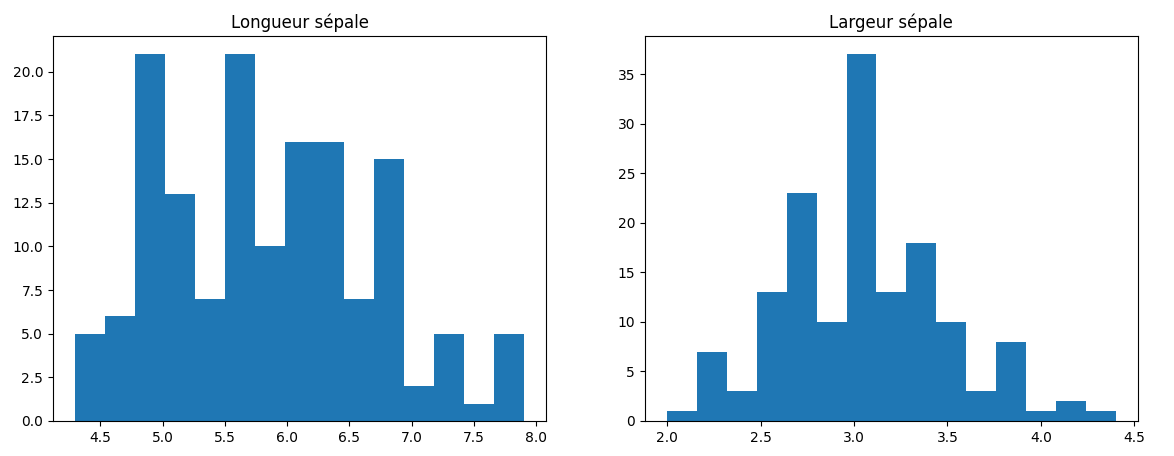
\includegraphics[width=\linewidth]{img/NBdistrib.png}
					\caption{Distribution des longueurs et largeurs des sépales}
				\end{figure}
				
\begin{lstlisting}[title=Progamme complet]
from sklearn.datasets import load_iris
from sklearn.model_selection import train_test_split
from sklearn.naive_bayes import GaussianNB
from sklearn.metrics import accuracy_score, confusion_matrix, ConfusionMatrixDisplay, f1_score, \
    recall_score

import matplotlib.pyplot as plt

X, y = load_iris(return_X_y=True)

X_train, X_test, y_train, y_test = train_test_split(X, y, test_size=0.33, random_state=0)
model = GaussianNB()
model.fit(X_train, y_train)

y_pred = model.predict(X_test)
precision = accuracy_score(y_pred, y_test)
recall = recall_score(y_test, y_pred, average="weighted")
f1 = f1_score(y_pred, y_test, average="weighted")

print("Precision:", precision)
print("Rappel:", recall)
print("Score F1:", f1)

plt.figure('Donnees du modele', figsize=(14, 5))
plt.subplot(1, 3, 1, title='Donnees du train set')
plt.scatter(X_train[:, 0], X_train[:, 1], c=y_train)
plt.xlabel('Sepale long.')
plt.ylabel('Sepale larg.')
plt.subplot(1, 3, 2, title='Donnees du test set')
plt.scatter(X_test[:, 0], X_test[:, 1], c=y_test)
plt.xlabel('Sepale long.')
plt.subplot(1, 3, 3, title='Donnees test apres evaluation')
plt.scatter(X_test[:, 0], X_test[:, 1], c=y_pred)
plt.xlabel('Sepale long.')
plt.show()

cm = confusion_matrix(y_test, y_pred, labels=[0, 1, 2])
disp = ConfusionMatrixDisplay(confusion_matrix=cm, display_labels=[0, 1, 2])
disp.ax_.set_title('Matrice de confusion')
disp.plot()
plt.show()

plt.figure('Distribution des donnees Iris', figsize=(14, 5))
plt.subplot(1, 2, 1, title='Longueur sepale')
plt.hist(X[:, 0], bins=15)
plt.subplot(1, 2, 2, title='Largeur sepale')
plt.hist(X[:, 1], bins=15)
plt.show()\end{lstlisting}
				
				Les données du dataset ont été séparés en 2 jeux, un pour l’entraînement du modèle et un pour le test. On obtient alors la représentation suivantes après entrainement et test du modèle
				\begin{figure}[H]
					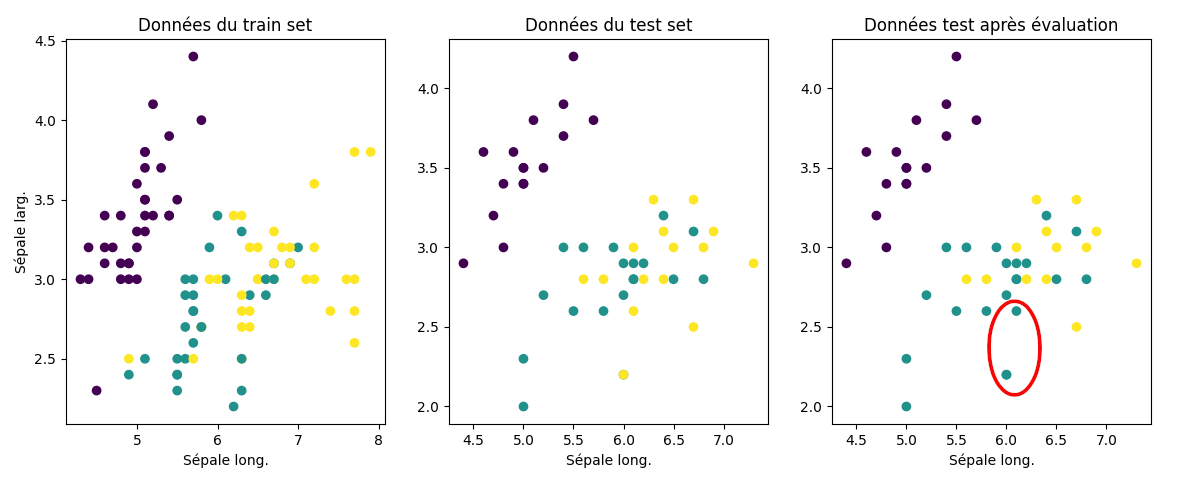
\includegraphics[width=\linewidth]{img/NBdata.png}
					\caption{Représentation des données }
				\end{figure}
				
				Dans les données de test nous avons 2 catégorisations qui n'ont pas été réalisées correctement. On obtient les scores suivants :
				\begin{itemize}
					\item Précision: 0.96                    \footnote{La précision est la proportion des éléments correctement identifiés sur l'ensemble des éléments prédit}
					\item Rappel: 0.96						\footnote{Le rappel est la proportion des éléments correctement identifiés sur l'ensemble des éléments de la catégorie}
					\item Score F1: 0.9604285714285714		\footnote{Le Score F1 est la moyenne harmonique calculée de la manière suivante $2*(precision*rappel)/(precision+rappel)$}
				\end{itemize}				
				
				\begin{figure}[H]
					\centering
					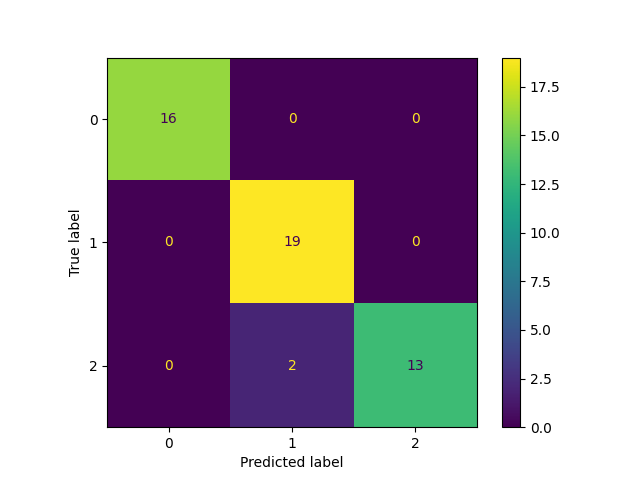
\includegraphics[scale=0.7]{img/NBmatrix.png}
					\caption{Matrice de confusion}
				\end{figure}
				
				A l'aide de ce modèle nous devrions avoir une 96\% de chance de déterminer la bonne variété d'iris en se basant sur la longueur et la largeur des sépales.  
				
			\paragraph{Avantages et inconvénients} 
				Le modèle Naïve Bayes est un modèle simple et rapide qui ne nécessite pas de grande capacités de calcul. De ce fait il permet de traiter une grande quantité de données.\\
				
				Cependant, les données qui lui sont fournies ne doivent pas être corrélées ce qui est rarement le cas dans les problèmes du monde réel. Ce type de modèle est limité à des problèmes de classification supervisée. Si on se fie à l'équation (\ref{NBeq}) la probabilité d'apparition de l’évènement B : P(B) ne peut pas être nulle. 
	
	
	\section{Bibliographie}
		\bibliographystyle{plain}
		\bibliography{IED_L3_Projet_Inglang_Fouille_IA}
		


		
	\section{Sitotec}
		\subsection{Corpus}
			\begin{itemize}
				\item Enron company mails, fichier CSV contenant l'ensemble des mails d'une entreprise ayant fermée ses portes (33.834.245 mails) [en ligne], \url{https://www.kaggle.com/wcukierski/enron-email-dataset} (consulté le 27/01/2022) \label{Enron_dataset}
				\item Mails project SpamAssassin, projet opensource de détection de spam (6065 fichiers email déjà trier en ham et spam) [en ligne], \url{https://spamassassin.apache.org/old/publiccorpus/} (consulté le 27/01/2022) \label{SpamAssassin_dataset}
				\item Brown corpus, ensemble de texte en anglais publié en 1961 qui contient plus d'un million de mots \url{https://www.nltk.org/book/ch02.html} (consulté le 20/08/2022) \label{Brown_corpus}
			\end{itemize}
		
		\subsection{Modules}
			\paragraph{Module langdetect}
			\begin{itemize}
				\item Page Github du projet \emph{langdetect} capable de différencier 49 langages avec une précision de 99\%, [en ligne] \url{https://github.com/Mimino666/langdetect} (consulté le 04/12/2022) \label{langdetect}
				\item Language Detection Library, présentation du module (anglais) [en ligne] \url{https://www.slideshare.net/shuyo/language-detection-library-for-java} (consulté le 04/12/2022)
			\end{itemize}
			
		\subsection{Modèles}
			\paragraph{Naïves Bayes}
				Le modèle Naïves Bayes est employé dans le module langdetect (\ref{langdetect})
			\begin{itemize}
				\item Les algorithmes de Naïves Bayes, Explication sommaire du principe de ces type d'algorithme, [en ligne] \url{https://brightcape.co/les-algorithmes-de-naives-bayes/} (consulté le 26/03/2023)
				\item Naive Bayes Classification Tutorial using Scikit-learn, exemple d'utilisation de ce type de modèle avec python (anglais) [en ligne] \url{https://www.datacamp.com/tutorial/naive-bayes-scikit-learn} (consulté le 26/03/2023)
				\item Scikit learn Naive Bayes, description des types d'algorithme disponibles dans le module Scikitlearn en python (anglais) [en ligne] \url{https://scikit-learn.org/stable/modules/naive_bayes.html} (consulté le 26/03/2023)
			\end{itemize}
	
	
\end{document}





















